\subsection{Visitor}
\subsubsection{Định nghĩa}
Visitor (Người ghé thăm) là một mẫu thiết kế hành vi cho phép thực hiện các thao tác trên các đối tượng của một tập hợp các lớp khác nhau mà không làm thay đổi cấu trúc của chúng. Mẫu này cho phép bạn định nghĩa các thao tác mới mà không phải thay đổi các lớp đã tồn tại và tách rời logic của các thao tác khỏi cấu trúc của các đối tượng.
\subsubsection{Cách sử dụng}
Ta có thể sử dụng Visitor Pattern trong các trường hợp sau:
\begin{itemize}
    \item Sử dụng khi cần thực hiện thao tác trên tất cả các phần tử của cấu trúc đối tượng phức tạp.
    \item Sử dụng khi một hành vi chỉ có ý nghĩa trong một số lớp của hệ thống phân cấp lớp, nhưng không có ý nghĩa trong các lớp khác.
    \item Khi có nhiều thao tác khác nhau cần thực hiện trên các đối tượng, và không muốn thay đổi các lớp của chúng.
\end{itemize}
\subsubsection{Cấu trúc}
\begin{center}
    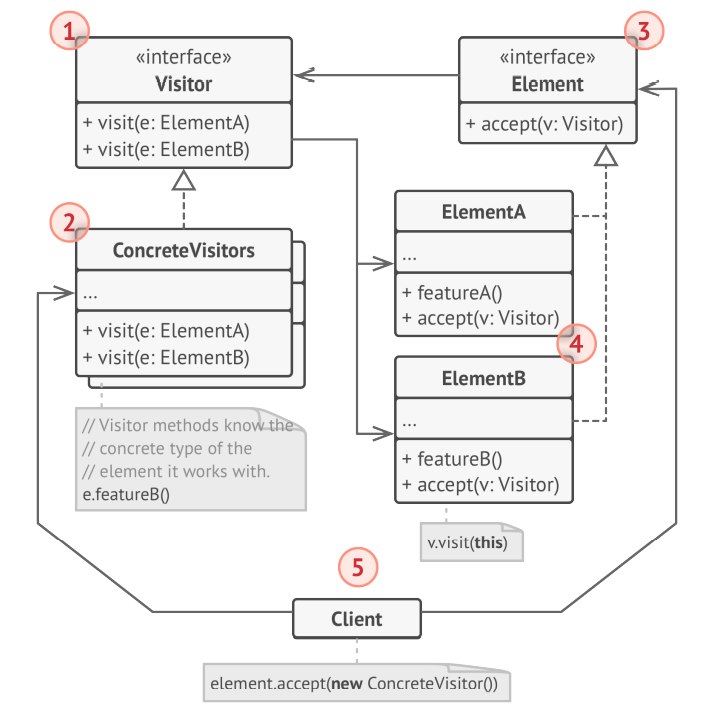
\includegraphics[scale=0.6]{image/behavioral/visitor.png}
\end{center}
\subsubsection{Ưu điểm và Nhược điểm}
Ta có rất nhiều ưu nhược điểm như sau:\\\\
Ưu điểm:
\begin{itemize}
    \item Một đối tượng visitor có thể tích lũy một số thông tin hữu ích khi làm việc với nhiều đối tượng khác nhau. Điều này có thể giúp ích khi ta muốn duyệt qua một số cấu trúc đối tượng phức tạp, chẳng hạn như cây đối tượng và áp dụng visitor cho từng đối tượng của cấu trúc này.
    \item Visitor cho phép tách rời logic của các thao tác khỏi cấu trúc của các đối tượng, giúp duy trì nguyên tắc đơn trách nhiệm (single responsibility principle).
    \item Visitor cho phép bạn thực hiện các thao tác khác nhau trên các đối tượng mà không cần thay đổi cấu trúc của chúng.
\end{itemize}
Nhược điểm:
\begin{itemize}
    \item Mẫu Visitor có thể làm tăng sự phức tạp của mã, đặc biệt khi có nhiều lớp và các thao tác phức tạp.
    \item Cần cập nhật tất cả visitor mỗi khi một lớp được thêm vào hoặc xóa khỏi hệ thống phân cấp phần tử.
    \item Các visitor có thể thiếu quyền truy cập cần thiết vào các trường riêng tư và phương thức của các phần tử mà họ phải làm việc với.
    \item Truyền đối tượng Visitor đến các đối tượng được ghé thăm có thể ảnh hưởng đến hiệu suất, đặc biệt khi có nhiều lớp và thao tác phức tạp.
\end{itemize}
\subsubsection{Code Example}
\begin{itemize}
    \item Có interface Element và 2 subclass.
    \item Có Abstract class Visitor và ConcreteVisitor.
\end{itemize}
\begin{lstlisting}
#include <iostream>
#include <vector>

// Forward declaration of classes
class ConcreteElementA;
class ConcreteElementB;

// Abstract Visitor class
class Visitor {
public:
    virtual void visit(ConcreteElementA* element) = 0;
    virtual void visit(ConcreteElementB* element) = 0;
};

// Abstract Element class
class Element {
public:
    virtual void accept(Visitor* visitor) = 0;
};

// Concrete Element A
class ConcreteElementA : public Element {
public:
    void accept(Visitor* visitor) override {
        visitor->visit(this);
    }

    std::string operationA() {
        return "ConcreteElementA";
    }
};

// Concrete Element B
class ConcreteElementB : public Element {
public:
    void accept(Visitor* visitor) override {
        visitor->visit(this);
    }

    std::string operationB() {
        return "ConcreteElementB";
    }
};

// Concrete Visitor
class ConcreteVisitor : public Visitor {
public:
    void visit(ConcreteElementA* element) override {
        std::cout << "ConcreteVisitor: Visit " << element->operationA() << std::endl;
    }

    void visit(ConcreteElementB* element) override {
        std::cout << "ConcreteVisitor: Visit " << element->operationB() << std::endl;
    }
};

int main() {
    // Create elements
    ConcreteElementA elementA;
    ConcreteElementB elementB;

    // Create visitor
    ConcreteVisitor visitor;

    // Accept visitor on elements
    elementA.accept(&visitor);
    elementB.accept(&visitor);

    return 0;
}

\end{lstlisting}
Ở hàm main, tạo ra 2 elements và một visitor cơ bản. Sau đó ta cho 2 elements này chấp nhận Visitor và cho ra kết quả.\\
\newline
\textbf{Kết quả:}
\begin{lstlisting}
ConcreteVisitor: Visit ConcreteElementA
ConcreteVisitor: Visit ConcreteElementB
\end{lstlisting}
\subsubsection{Các Pattern liên quan}
\begin{itemize}
    \item Một phiên bản hiệu quả của Command.
    \item Dùng Visitor để thực hiện thao tác trên cây Composite.
    \item Kết hợp với Iterator để duyệt qua cấu trúc dữ liệu phức tạp và thực hiện một vài Operation trên các phần tử của nó.
\end{itemize}